%!TEX root = ../Main.tex

\chapter{PolyMarker: A fast polyploid primer design pipeline}
\section{Introduction} 
%Explain how the SNP markers are designed without the tool and an overview. 


\begin{figure}
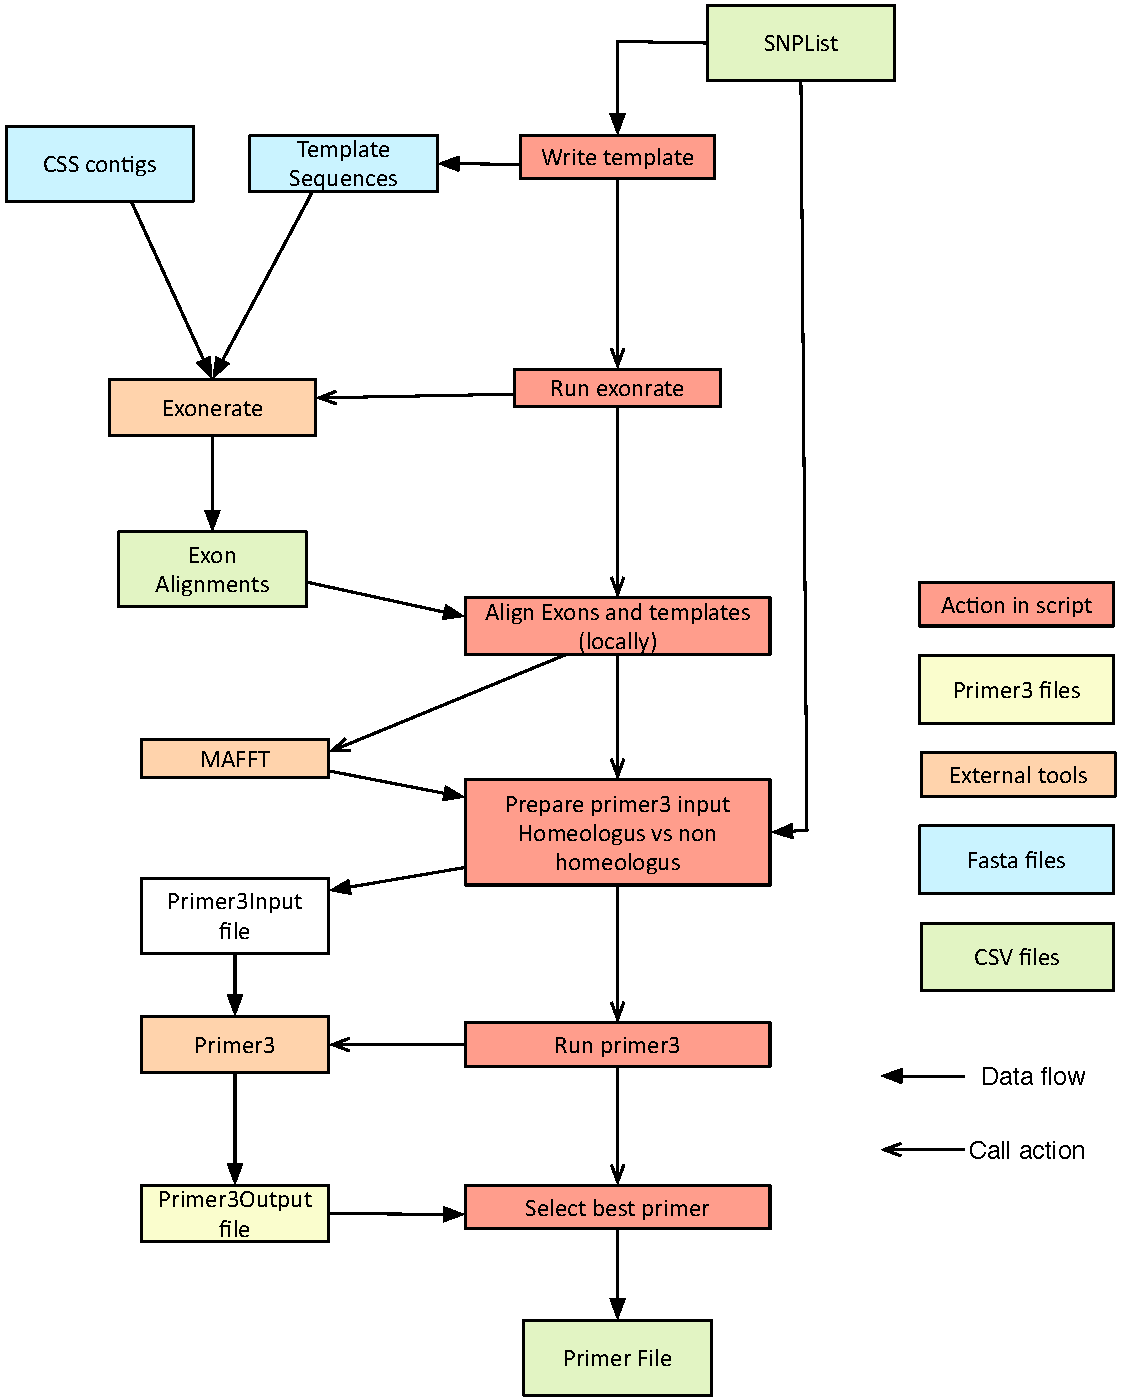
\includegraphics[width=1\textwidth]{PolyMarker/Figures/pipeline.pdf}
        \caption{PolyMarker Pipeline}
        \label{fig:poly:pipeline}
\end{figure}


\section{Global alignment} 
Search of the contigs with the sequence in the CSS reference and the importance of being able to distinguish between homoeologous regions. 


\begin{figure}
    \centering
    \begin{subfigure}[b]{0.4\textwidth}
        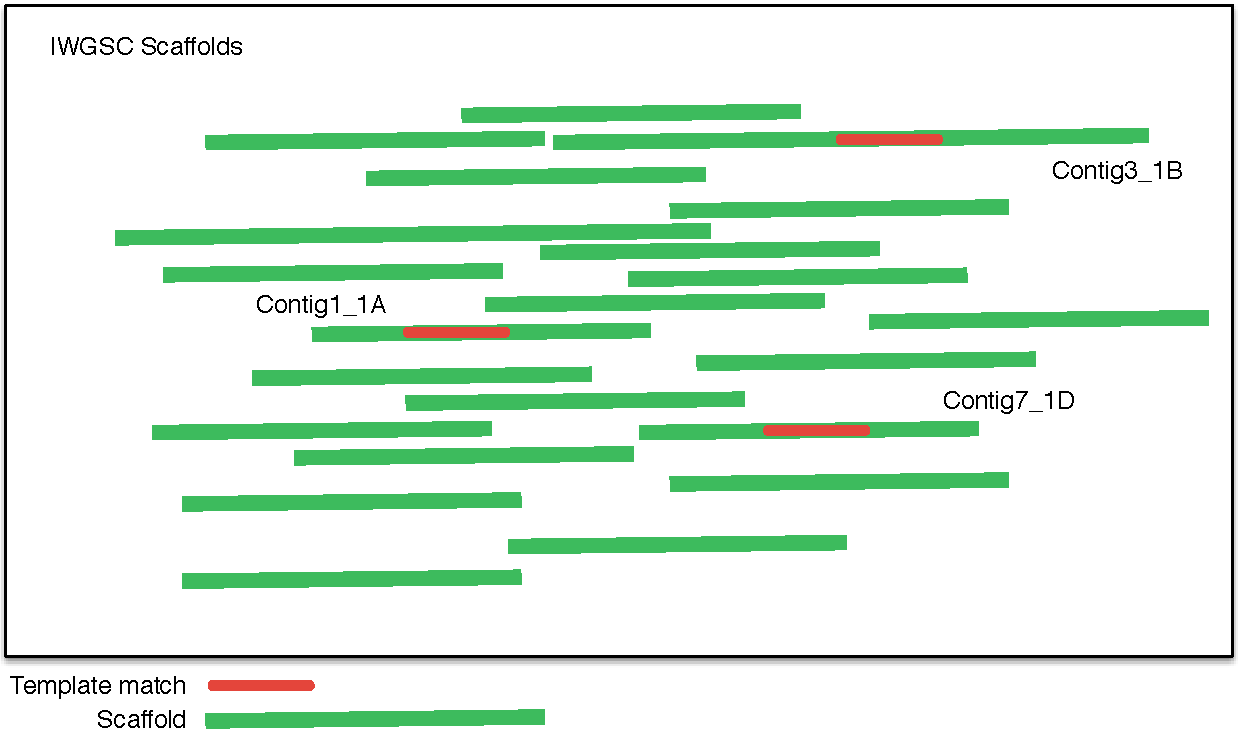
\includegraphics[width=1\textwidth]{PolyMarker/Figures/aln/scaffoldsSearch.pdf}
        \caption{Global search.}
        \label{fig:poly:globalSearch}
    \end{subfigure}
    ~ %add desired spacing between images, e. g. ~, \quad, \qquad, \hfill etc. 
      %(or a blank line to force the subfigure onto a new line)
    \begin{subfigure}[b]{0.4\textwidth}
        \raisebox{10mm} { 
\includegraphics[width=1\textwidth]{PolyMarker/Figures/aln/scaffoldsFoundAround.pdf} }
        \caption{Selected regions around the SNP on every chromosome.}
        \label{fig:poly:globalAround}
    \end{subfigure}
    
    \begin{subfigure}[b]{0.4\textwidth}
        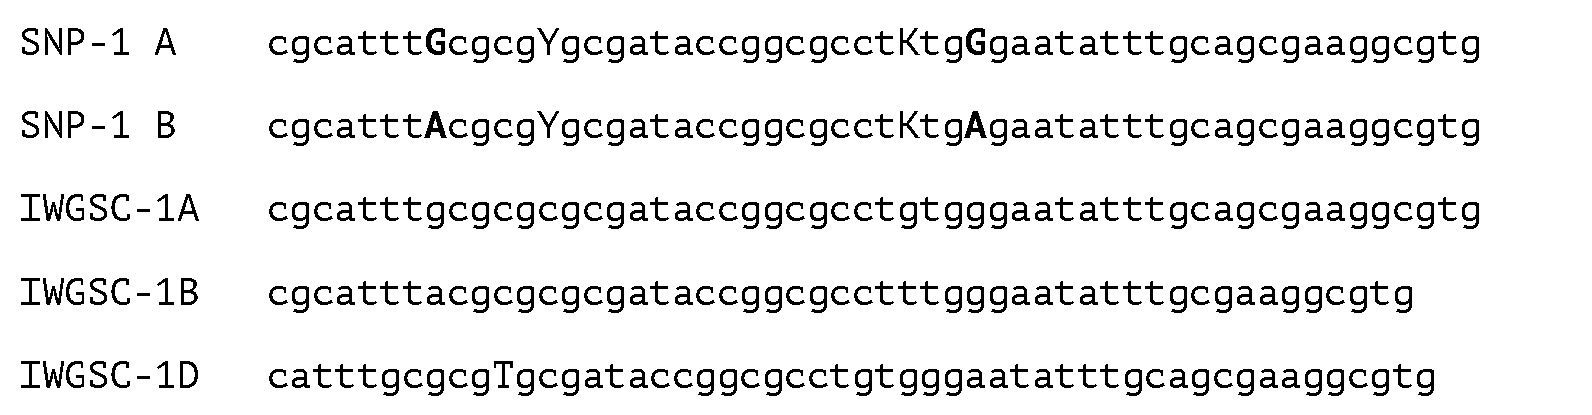
\includegraphics[width=1\textwidth]{PolyMarker/Figures/aln/scaffoldsFound.pdf}
        \caption{Sequence of found regions around the SNP.}
        \label{fig:poly:globalSequence}
    \end{subfigure}
    ~ %add desired spacing between images, e. g. ~, \quad, \qquad, \hfill etc. 
      %(or a blank line to force the subfigure onto a new line)
    \begin{subfigure}[b]{0.4\textwidth}
        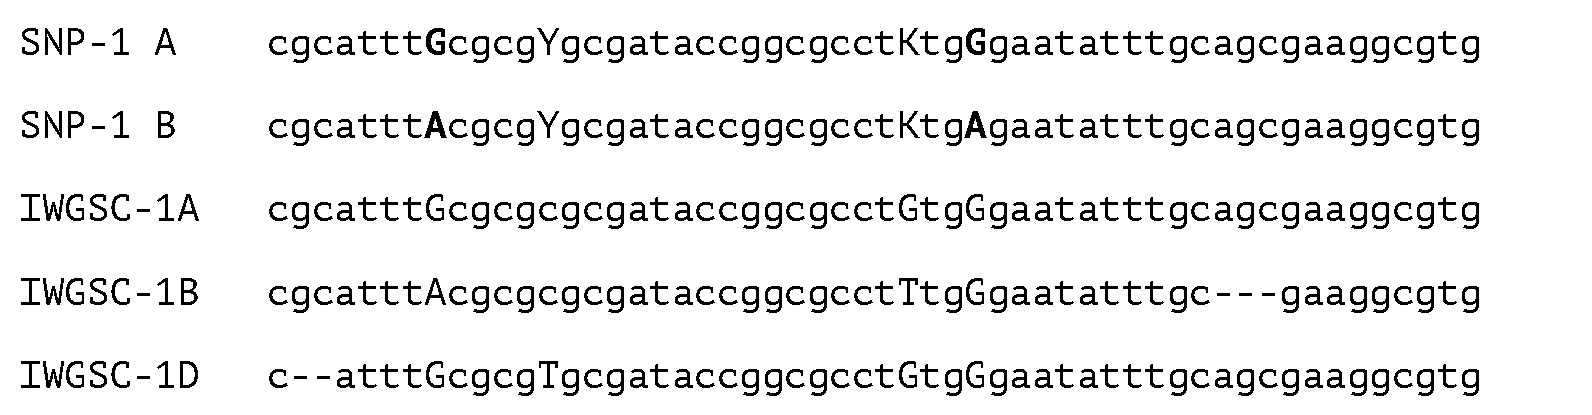
\includegraphics[width=1\textwidth]{PolyMarker/Figures/aln/localAlignment.pdf} 
        \caption{Local alignment on regions around the SNP to detect indels.}
        \label{fig:poly:localSequence}
    \end{subfigure}

    \begin{subfigure}[b]{0.8\textwidth}
        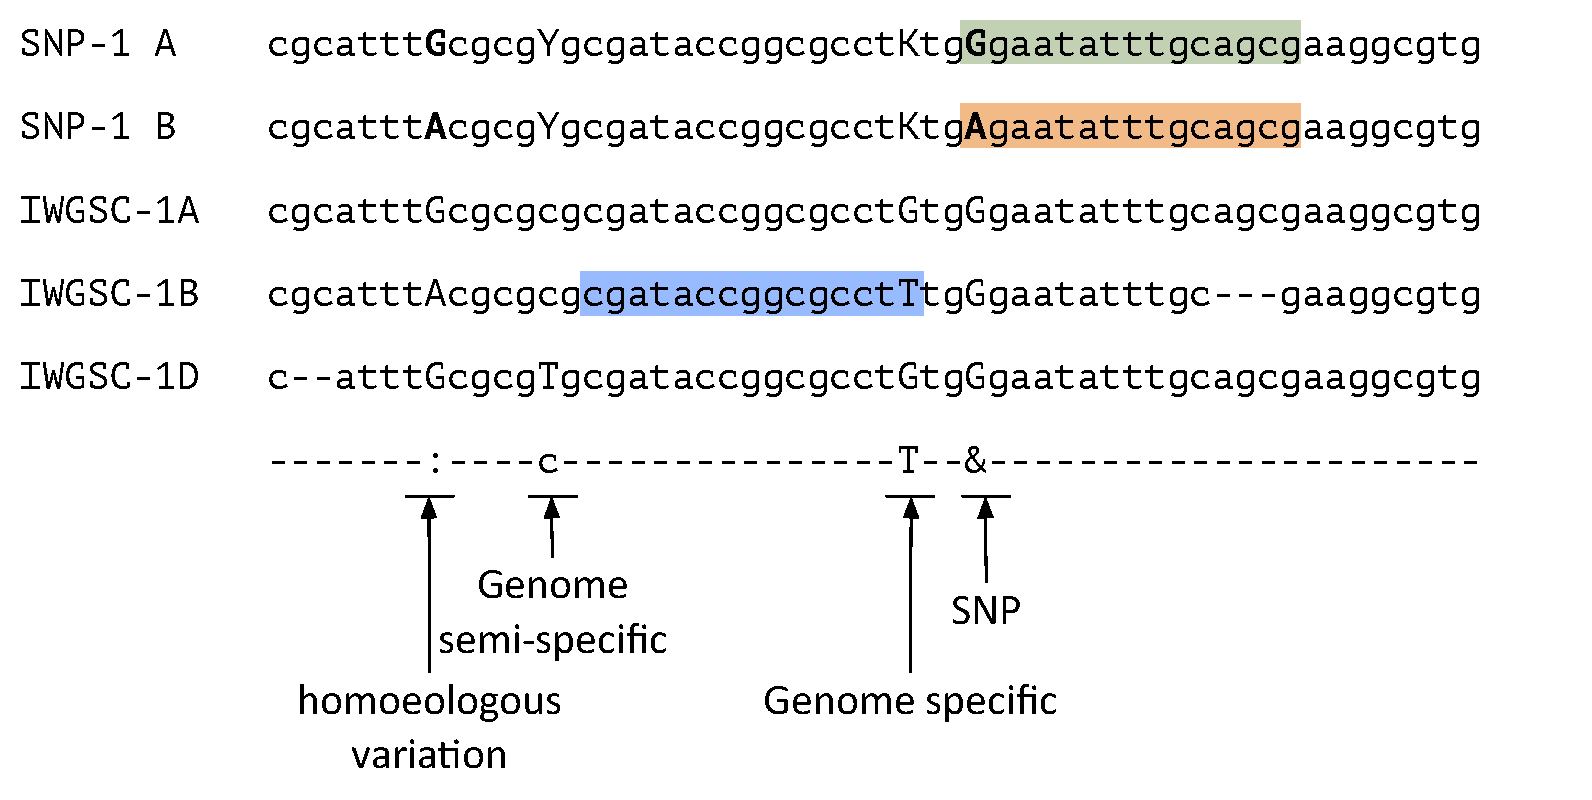
\includegraphics[width=1\textwidth]{PolyMarker/Figures/aln/mask.pdf} 
        \caption{Alignment with mask and primer candidates.}
        \label{fig:poly:mask}

    \end{subfigure}
    \caption{Alignments done by PolyMarker.}\label{fig:global}
\end{figure}

\section{Local alignment} 
Once the region with the primer has been selected, make a local alignment. This section discusses why the local alignment is needed. 

\section{Primer design tools} 
In this section, the principles of \textit{in silico} primer design are discussed, and why not simply selecting a genomic variation is enough (thermal stability, primers folding on themselves)

\section{Primer selection algorithms} 
Different algorithms to select the \"best primer\". 

\subsection{KASP markers} 
For KASP markers, the product should be as short as possible with the mutation in the first three bases. 

\section{Designed markers} Details of the generated primers for the 80k iSelect chip and the 820k axiom chip. This section also include counts on how many are genome specific, semi-specific and non specific. Also an analysis of how many are repeated or map to more than one chromosome perfectly.

\subsection{Regular markers}  
PolyMarker was designed for KASP assays, but it was later extended to produce regular primers, where both primers start with a genome-specific base. This simplifies the design of primers for regular PCR and capillary sequencing. 




\subsection{Deletion algorithms}
Algorithm to produce KASP for deletions in polyploids. 

\begin{figure}
    \centering
    \begin{subfigure}[b]{0.4\textwidth}
        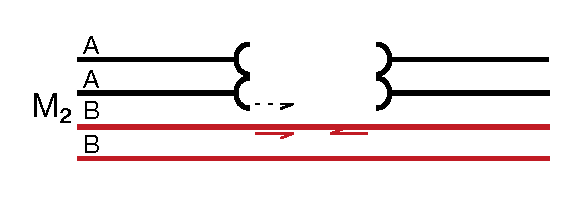
\includegraphics[width=1\textwidth]{PolyMarker/Figures/deletions/homM2.pdf}
        \caption{Homozygous deletion on $M_{2}$}
        \label{fig:poly:homM2}
    \end{subfigure}
    ~ %add desired spacing between images, e. g. ~, \quad, \qquad, \hfill etc. 
      %(or a blank line to force the subfigure onto a new line)
    \begin{subfigure}[b]{0.4\textwidth}
        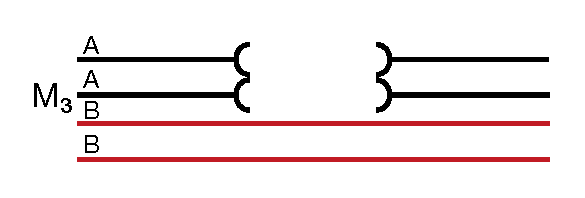
\includegraphics[width=1\textwidth]{PolyMarker/Figures/deletions/homM3.pdf} 
        \caption{Homozygous deletion on  $M_{3}$}
        \label{fig:poly:homM3}
    \end{subfigure}
    
    \begin{subfigure}[b]{0.3\textwidth}
        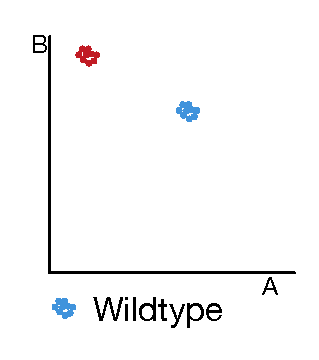
\includegraphics[width=1\textwidth]{PolyMarker/Figures/deletions/homReal.pdf}
        \caption{KASP amplification for a real deletion}
        \label{fig:poly:homReal}
    \end{subfigure}
    ~ %add desired spacing between images, e. g. ~, \quad, \qquad, \hfill etc. 
      %(or a blank line to force the subfigure onto a new line)
    \begin{subfigure}[b]{0.3\textwidth}
        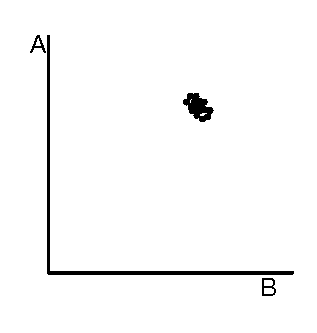
\includegraphics[width=1\textwidth]{PolyMarker/Figures/deletions/homFalse.pdf} 
        \caption{KASP amplification on false positive}
        \label{fig:poly:homFalse}
    \end{subfigure}
    \begin{subfigure}[b]{0.3\textwidth}
        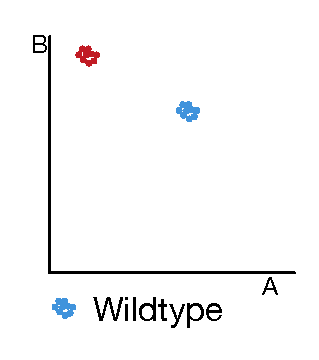
\includegraphics[width=1\textwidth]{PolyMarker/Figures/deletions/homReal.pdf} 
        \caption{Example of validated deletion on mutant poulation}
        \label{fig:poly:homTest}
    \end{subfigure}
    \caption{PolyMarker used to find primers to detect long deletions in tetraploid wheat.}
    \label{fig:poly:homDel}
\end{figure}



\section{Conclusions} Remarks on the importance of getting the primers right, and the time saved by automating the primer selection. Also mention other primer design tools that have been inspired by polymarker: \cite{Ma2015}, \cite{Wang2016}

PolyMarker has been used succesfully to design genome-specific primers in several projects. 


